\specialchapter{\texorpdfstring{图版 V. \(E_{6}\) 型根系}{图版 V. E\_6 型根系}}

\begin{enumerate}
\def\labelenumi{(\Roman{enumi})}
\tightlist
\item
  V 是 \(E = R^{8}\) 的子空间，由坐标 \((\xi_{i})\) 满足 \(\xi_{6} = \xi_{7} = -\xi_{8}\) 的点组成。根：\(\pm\varepsilon_{i} \pm \varepsilon_{j} (1 \leqslant i < j \leqslant 5)\)，
\end{enumerate}

\[
\pm \frac {1}{2} (\varepsilon_ {8} - \varepsilon_ {7} - \varepsilon_ {6} + \sum_ {i = 1} ^ {5} (- 1) ^ {\nu (i)} \varepsilon_ {i}) \text {with} \sum_ {i = 1} ^ {5} \nu (i) \text {even.}
\]

根的数目：n = 72。

\begin{enumerate}
\def\labelenumi{(\Roman{enumi})}
\setcounter{enumi}{1}
\tightlist
\item
  基：\(\alpha_{1} = \frac{1}{2} (\varepsilon_{1} + \varepsilon_{8}) - \frac{1}{2} (\varepsilon_{2} + \varepsilon_{3} + \varepsilon_{4} + \varepsilon_{5} + \varepsilon_{6} + \varepsilon_{7}),\alpha_{2} = \varepsilon_{1} + \varepsilon_{2},\alpha_{3} =\) \(\varepsilon_2 - \varepsilon_1,\alpha_4 = \varepsilon_3 - \varepsilon_2,\alpha_5 = \varepsilon_4 - \varepsilon_3,\alpha_6 = \varepsilon_5 - \varepsilon_4.\) 正根：\(\pm \varepsilon_i + \varepsilon_j\) \(1\leqslant i <   j\leqslant 5)\)
\end{enumerate}

\[
\frac {1}{2} \left(\varepsilon_ {8} - \varepsilon_ {7} - \varepsilon_ {6} + \sum_ {i = 1} ^ {5} (- 1) ^ {\nu (i)} \varepsilon_ {i}\right) \text {with} \sum_ {i = 1} ^ {5} \nu (i) \text {even}.
\]

至少有一个系数 \(\geqslant 2\) 的正根（我们把根 \(a\alpha_{1} + b\alpha_{2} + c\alpha_{3} + d\alpha_{4} + e\alpha_{5} + f\alpha_{6}\) 记为 \({ }^{a c d e f}_{b})^{13}\)：

\[
\begin{array}{c c c c c c} 0   1   2   1   0 & 1   1   2   1   0 & 0   1   2   1   1 & 1   2   2   1   0 & 1   1   2   1   1 & 0   1   2   2   1 \\ 1 & 1 & 1 & 1 & 1 & 1 \\ 1   2   2   1   1 & 1   1   2   2   1 & 1   2   2   2   1 & 1   2   3   2   1 & 1   2   3   2   1 \\ 1 & 1 & 1 & 1 & 2 \end{array}
\]

\begin{enumerate}
\def\labelenumi{(\Roman{enumi})}
\setcounter{enumi}{2}
\item
  Coxeter 数：\(h = 12\) 。
\item
  最高根：
\end{enumerate}

\[
\begin{array}{r l} \tilde {\alpha} & = \frac {1}{2} (\varepsilon_ {1} + \varepsilon_ {2} + \varepsilon_ {3} + \varepsilon_ {4} + \varepsilon_ {5} - \varepsilon_ {6} - \varepsilon_ {7} + \varepsilon_ {8}) \\ & = \alpha_ {1} + 2 \alpha_ {2} + 2 \alpha_ {3} + 3 \alpha_ {4} + 2 \alpha_ {5} + \alpha_ {6} = \omega_ {2}. \end{array}
\]

扩展 Dynkin 图：

\pandocbounded{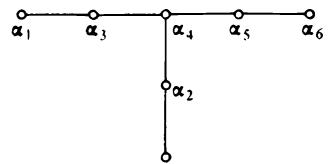
\includegraphics[keepaspectratio]{images/part002_985a73c0.jpg}}

\begin{enumerate}
\def\labelenumi{(\Alph{enumi})}
\setcounter{enumi}{21}
\tightlist
\item
  \(R^{\prime} = R.\)
\end{enumerate}

\[
  \Phi_ {\mathrm{R}} (x, y) = (x | y) / 24, \quad \gamma (\mathrm{R}) = 144.
\]

\begin{enumerate}
\def\labelenumi{(\Roman{enumi})}
\setcounter{enumi}{5}
\tightlist
\item
  基本权：
\end{enumerate}

\[
\begin{array}{l} \omega_ {1} = \frac {2}{3} (\varepsilon_ {8} - \varepsilon_ {7} - \varepsilon_ {6}) = \frac {1}{3} (4 \alpha_ {1} + 3 \alpha_ {2} + 5 \alpha_ {3} + 6 \alpha_ {4} + 4 \alpha_ {5} + 2 \alpha_ {6}) \\ \omega_ {2} = \frac {1}{2} (\varepsilon_ {1} + \varepsilon_ {2} + \varepsilon_ {3} + \varepsilon_ {4} + \varepsilon_ {5} - \varepsilon_ {6} - \varepsilon_ {7} + \varepsilon_ {8}) \\ \quad = \alpha_ {1} + 2 \alpha_ {2} + 2 \alpha_ {3} + 3 \alpha_ {4} + 2 \alpha_ {5} + \alpha_ {6} = \tilde {\alpha} \\ \omega_ {3} = \frac {5}{6} (\varepsilon_ {8} - \varepsilon_ {7} - \varepsilon_ {6}) + \frac {1}{2} (- \varepsilon_ {1} + \varepsilon_ {2} + \varepsilon_ {3} + \varepsilon_ {4} + \varepsilon_ {5}) \\ \quad = \frac {1}{3} (5 \alpha_ {1} + 6 \alpha_ {2} + 10 \alpha_ {3} + 12 \alpha_ {4} + 8 \alpha_ {5} + 4 \alpha_ {6}) \\ \omega_ {4} = \varepsilon_ {3} + \varepsilon_ {4} + \varepsilon_ {5} - \varepsilon_ {6} - \varepsilon_ {7} + \varepsilon_ {8} \\ \quad = 2 \alpha_ {1} + 3 \alpha_ {2} + 4 \alpha_ {3} + 6 \alpha_ {4} + 4 \alpha_ {5} + 2 \alpha_ {6} \\ \omega_ {5} = \frac {2}{3} (\varepsilon_ {8} - \varepsilon_ {7} - \varepsilon_ {6}) + \varepsilon_ {4} + \varepsilon_ {5} \\ \quad = \frac {1}{3} (4 \alpha_ {1} + 6 \alpha_ {2} + 8 \alpha_ {3} + 12 \alpha_ {4} + 10 \alpha_ {5} + 5 \alpha_ {6}) \\ \omega_ {6} = \frac {1}{3} (\varepsilon_ {8} - \varepsilon_ {7} - \varepsilon_ {6}) + \varepsilon_ {5} \\ \quad = \frac {1}{3} (2 \alpha_ {1} + 3 \alpha_ {2} + 4 \alpha_ {3} + 6 \alpha_ {4} + 5 \alpha_ {5} + 4 \alpha_ {6}). \end{array}
\]

\begin{enumerate}
\def\labelenumi{(\Roman{enumi})}
\setcounter{enumi}{6}
\tightlist
\item
  正根之和：
\end{enumerate}

\[
\begin{array}{l} 2 \rho = 2 (\varepsilon_ {2} + 2 \varepsilon_ {3} + 3 \varepsilon_ {4} + 4 \varepsilon_ {5} + 4 (\varepsilon_ {8} - \varepsilon_ {7} - \varepsilon_ {6})) \\ = 2 (8 \alpha_ {1} + 11 \alpha_ {2}) + 15 \alpha_ {3} + 21 \alpha_ {4} + 15 \alpha_ {5} + 8 \alpha_ {6}). \end{array}
\]

\begin{enumerate}
\def\labelenumi{(\Roman{enumi})}
\setcounter{enumi}{7}
\tightlist
\item
  P(R)/Q(R) 同构于 Z/3Z。
\end{enumerate}

连接指标：3。

\begin{enumerate}
\def\labelenumi{(\Roman{enumi})}
\setcounter{enumi}{8}
\item
  指数：1, 4, 5, 7, 8, 11。
\item
  W(R) 的阶：\(2^{7}.3^{4}.5\) 。
\item
  \(\mathrm{A}(\mathrm{R}) = \mathrm{W}(\mathrm{R}) \times \{1, -1\}\)；\(w_0\) 分别将 \(\alpha_1, \alpha_2, \alpha_3, \alpha_4, \alpha_5, \alpha_6\) 变为 \(-\alpha_6, -\alpha_2, -\alpha_5, -\alpha_4, -\alpha_3, -\alpha_1\)。
\item
  \(\mathrm{A}(\mathbb{R}) / \mathrm{W}(\mathbb{R})\) 的非恒等元确定自同构 \(x \mapsto -x\) 在 \(\mathrm{P}(\mathbb{R}) / \mathrm{Q}(\mathbb{R})\) 上的作用。
\end{enumerate}

扩展 Dynkin 图的自同构群同构于 \(S_{3}\)；其阶为 3 的元素由 \(P(R^{-})/Q(R^{-})\) 的两个非平凡元诱导。

\[
\left( \begin{array}{c c c c c c} 2 & 0 & - 1 & 0 & 0 & 0 \\ 0 & 2 & 0 & - 1 & 0 & 0 \\ - 1 & 0 & 2 & - 1 & 0 & 0 \\ 0 & - 1 & - 1 & 2 & - 1 & 0 \\ 0 & 0 & 0 & - 1 & 2 & - 1 \\ 0 & 0 & 0 & 0 & - 1 & 2 \end{array} \right)
\]

\begin{enumerate}
\def\labelenumi{(\Roman{enumi})}
\setcounter{enumi}{12}
\tightlist
\item
  Cartan 矩阵：
\end{enumerate}

